

\StartOf{Lecture 5}

\Today{(0) Sampling from L4, (1) Intro to PAM, (2) ISI / Nyquist Filtering Theorem}

\announcements{
\begin{itemize}
  \item Today:  Rice A.2, 3.2.  For Wed: Rice 5.2, 5.3
  \item HW 2 due Thursday 11:59pm (extended one day).  Late deadline of Friday 11:59pm.
  \item Project 1 due Monday a week from today at 11:59pm. First 4 projects have been postponed by one week.
  \item Office hours: Mon 2:30-4pm, Tue 11-noon at Kaldi's coffee (Skinker and Forest Park Parkway)
  \item Keren Li (our AI) will have office hours weekly, Wed 4-5pm, location t.b.a.
\end{itemize}
}

\section{Intro to PAM}

Pulse amplitude modulation is a one-dimensional modulation, that is, it has one waveform $\phi_0(t)$.  We write this as $\phi_0(t) = p(t)$, where $p(t)$ is a unit-energy waveform called the pulse shape.  (The reason to use $p(t)$ will become clear later when we introduce other modulations.)  To encode symbols, we will choose an amplitude $a_{m,0}$ to indicate the $m$th symbol, and make the $a_{m,0}$ different.  For example, for $M=2$, we might choose amplitudes $\{-A, A\}$ (this is also called binary bipolar PAM).  The variable $A$ then determines the energy of the symbol.  As another example, for $M=4$, we could choose from the set $\{-3A, -A, A, 3A\}$.  These are equally spaced, but for $M> 2$, different symbols have different energies.  In particular, for $M$-PAM, the constellation diagram is shown in Rice Section 5.2.1, %Figure 5.2.1 (??), 
and amplitudes $\{a_{m,0}\}_m$ are,
\[
 -(M-1)A, -(M-3)A, \ldots, -A, A, \ldots, (M-3)A, (M-1)A
\]
The average energy, assuming that each symbol is equally likely, can be shown to be:
\[
 E_{avg} = \frac{M^2-1}{3}A^2
\]

To send multiple symbols over time, we transmit a signal $s(t)$,
\[
 s(t) = \sum_n a(n) p(t-nT_s),
\]
where $a(n)$ is the amplitude (one of the $\{a_{m,0}\}_m$) of the $n$th symbol we choose to send, and $T_s$ is the symbol period.  Each subsequent pulse is delayed in time by $T_s$.  


\Example{Binary Bipolar PAM} Figure \ref{F:PAM-binary-square-pulse}
shows a 4-ary PAM signal set using amplitudes $a_{0,0}=-A$, $a_{1,0} = A$.
It shows a signal set using square pulses,
\[
  \phi_0(t) = p(t) = \pdfarray{1/\sqrt{T_{s}}}{0 \le t < T_{s}}
\]
  \begin{figure}[htbp]
    \centerline{\includegraphics[width=0.6\textwidth]{../images/PAM-binary-square-pulse.eps} }
    \caption{Example signal for binary bipolar PAM example for $A = \sqrt{T_{s}}$.}
    \label{F:PAM-binary-square-pulse}
  \end{figure}


At the receiver, what we do is multiply the received signal $r(t)$ by $\phi_0(t)$ and integrate:
\[
 x = \int_{t=-\infty}^\infty r(t) \phi_0(t) dt
\]
This is also called \emph{correlation}. This needs to happen at each multiple of $T_s$. 
But there really are finite limits -- let's say that the signal has
a duration $T_s$, and then rewrite the integral as
\begin{equation} \label{E:Correlation}
 x = \int_{t=0}^{T_s} r(t) \phi_0(t) dt
\end{equation}
Essentially, this is as if we had multiple orthogonal waveforms, and thus our receiver is a bunch of parallel correlations, each time delayed by $T_s$, as shown in Figure \ref{F:multiple_correlation}.  Note that my integral limits in Figure \ref{F:multiple_correlation} may be wider if the pulse is wider than $T_s$ (e.g., the $n$th branch would start before $nT_s$ and end after $(n+1)T_s$).

  \begin{figure}[htbp]
    \centerline{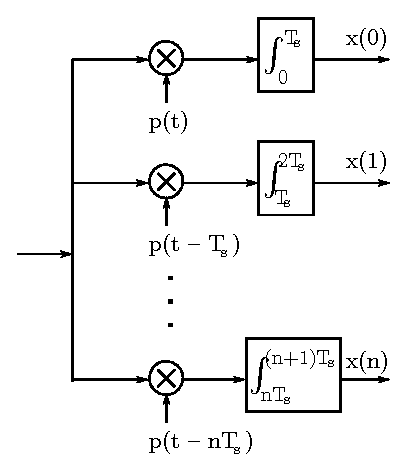
\includegraphics[width=0.5\textwidth]{../images/time_delay_correlation_receiver.eps} }
    \caption{The pulse shape $p(t)$ is chosen to be orthogonal to itself at integer multiples of the time delay.  Thus a PAM receiver might be implemented as a correlation receiver, in which each correlation (multiplication and integration) is done in parallel.}
    \label{F:multiple_correlation}
  \end{figure}
  
In reality, instead of a correlation, we can equivalently do a matched filter.  Equation (\ref{E:Correlation}) can be written as
\[
 x = \int_{t=0}^{T_s} r(t) h(T_s - t) dt
\]
where $h(t) = \phi_0(T_s-t)$.  (Plug in $(T_s-t)$ in this formula and
the $T_s$s cancel out and only positive $t$ is left.)  This is the
output of a convolution, taken at time $T_s$,
\[
 x =  \left. r(t) \star h(t) \right|_{t=T_s}
\]
Or equivalently
\[
 x =  \left. r(t) \star \phi_0(T_s-t) \right|_{t=T_s}
\]

  \begin{figure}[htbp]
    \centerline{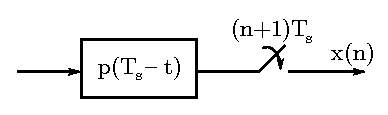
\includegraphics[width=0.45\textwidth]{../images/matched_filter_receiver.eps} }
    \caption{A matched filter receiver inputs $r(t)$ to a filter with impulse response $p(T_s-t)$, and then samples the output each multiple of $T_s$.}
    \label{F:matched_filter_rx}
  \end{figure}

Notes:
\begin{itemize}
  \item $x(n)$ is the output of a matched filter at time $nT_s$.
  \item We might, for example, have a physical filter with the impulse
    response $\phi_0(T_s-t)$, in which case it would be easy to do a matched filter
    implementation.
\end{itemize}

Try out the Matlab code,
\texttt{correlation\_and\_matched\_filter\_rx.m}, which is posted on
Canvas, for some examples of a pulse shape, adding noise, and performing the filtering for a correlation and matched filter receiver.


\section{Inter-Symbol Interference (ISI)}


\begin{enumerate}
  \item Consider the spectrum of the ideal 1-D PAM system with a square pulse.
  \item Consider the time-domain of the signal which is close to a rect function in the frequency domain.
\end{enumerate}
We don't want either:  (1) the pulse occupies too much spectrum, and (2) the pluse occupies too much time.
\begin{enumerate}
  \item If we try (1) above and use FDMA (frequency division
  multiple access) then the interference is \emph{out-of-band
  interference}.
  \item If we try (2) above and put symbols right next to each other in time, our
  own symbols experience interference called \emph{inter-symbol
  interference}.
\end{enumerate}

In reality, we want to compromise between (1) and (2) and experience
only a small amount of both.




\subsection{Nyquist Filtering}

We want to extend the pulse $p(t)$ to be longer in duration than only between zero and $T_s$, but we want to do so in a way that preserves the property that $p(t)$ and $p(t-T_s)$, and for that matter, $p(t-nT_s)$ for integers $n\neq 0$, are orthogonal.

Key insight:  we don't need $p(t)$ and $p(t-\tau)$ to be orthogonal for all real-valued times $\tau$ -- only for $\tau = nT_{s}$, for integer $n$.  In other words, the set:
\[
 \ldots,p(t+2T_s), p(t+T_s), p(t), p(t-T_s), p(t-2T_s), \ldots
\]
form an orthonormal set.  The Nyquist filtering condition is a frequency-domain rule that can be used to design arbitrary pulse shapes $p(t)$ that meet this condition.


\Theorem{Nyquist Filtering}{Let $r_p(t) = \intinfty{\tau}{p(\tau)p(\tau-t)}$ be the autocorrelation function of pulse shape $p(t)$.  A necessary and sufficient condition for
$r_p(t)$ to satisfy
\[
  r_p(nT_{s}) = \pdfarray{1}{n=0}
\]
is that its Fourier transform $R_p(f)$ satisfy
\[
  \sum_{m=-\infty}^\infty R_p\left(f + \frac{m}{T_{s}}\right) = T_{s}
\]
}{Proof: on page 677, Appendix A, of Rice book.}

Basically, $R_p(f)$ could be:
\begin{itemize}
  \item $R_p(f) = \rect(fT_{s})$, \ie, exactly constant within $-\frac{1}{2T_{s}} < f < \frac{1}{2T_{s}}$ band
  and zero outside.
  \item It may bleed into the next `channel' but the sum of
    \[ \cdots + R_p\left(f - \frac{1}{T_{s}}\right) + R_p(f) +
          R_p\left(f + \frac{1}{T_{s}}\right) + \cdots \]
    must be constant across all $f$.
\end{itemize}
Thus $R_p(f)$ is allowed to bleed into other frequency bands -- but
the neighboring frequency-shifted copy of $R_p(f)$ must be lower s.t.
the sum is constant.  See Figure \ref{F:NyquistFiltering}.

\begin{figure}[htbp]
\centerline{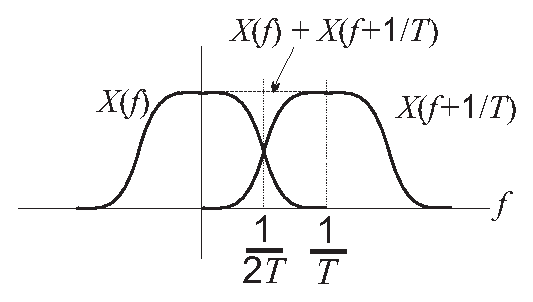
\includegraphics[width=0.7\textwidth]{../images/NyquistFiltering.eps}}
\caption{The Nyquist filtering criterion --
$1/T_{s}$-frequency-shifted copies of $R_p(f)$ must add up to a
constant.}\label{F:NyquistFiltering}
\end{figure}

If $R_p(f)$ only bleeds into one neighboring channel (that is, $R_p(f) =
0$ for all $|f| > \frac{1}{T_{s}}$), we denote the difference
between the ideal rect function and our $R_p(f)$ as $\Delta(f)$,
\[
  \Delta(f) = \left| R_p(f) - \rect(fT_{s}) \right|
\]
then we can rewrite the Nyquist Filtering condition as,
\[
   \Delta\left( \frac{1}{2T_{s}} - f \right) = \Delta\left( \frac{1}{2T_{s}} + f \right)
\]
for $-1/T_{s} \le f < 1/T_{s}$.  Essentially, symmetric about
$f=1/(2T_{s})$. See Figure \ref{F:NyquistFiltering}

Bateman presents this whole condition as ``A Nyquist channel
response is characterized by the transfer function having a
transition band that is symmetrical about a frequency equal to $0.5
\times 1/T_{s}$.''

\vspace{0.1in} \noindent {\bf Activity:}  Do-it-yourself Nyquist filter.  Take a sheet of paper and fold it in half, and then in half the other direction.  Cut a function in the thickest side (the edge that you just folded).  Leave a tiny bit so that it is not completely disconnected into two halves.  Unfold.  Drawing a horizontal line for the frequency $f$  axis, the middle is $0.5/T_s$, and the vertical axis it $R_p(f)$. One half (bottom or top) will be a plot of $R_p(f)$, and the other half will be an (inverse) plot of $R_p(f-T_s)$.


\subsection{Square Root Raised Cosine Pulse Shapes}

The raised-cosine function is given by:
\begin{equation} \label{E:RC}
H_{RC}(f) = \pdfarrays{T_{s}}{0 \le |f| \le
\frac{1-\alpha}{2T_{s}}}
                      {\frac{T_{s}}{2}\left\{ 1 + \cos \left[
                      \frac{\pi T_{s}}{\alpha} \left( |f| - \frac{1-\alpha}{2T_{s}}
                       \right)\right]\right\}}{ \frac{1-\alpha}{2T_{s}} \le |f| \le
                       \frac{1+\alpha}{2T_{s}}}
\end{equation}
Note that this is the $R_p(f)= H_{RC}(f)$ that meets the Nyquist filtering condition.  The pulse shape $p(t)$ must be such that $r_p(t)$, the autocorrelation function, has the Fourier transform $R_p(t)$.  How do we get that?  Well, recall that convolution in the time domain is multiplication in the frequency domain.  And autocorrelation (correlation with the same function itself) then is squaring in the frequency domain.  Thus $r_p(t) = \intinfty{\tau}{p(\tau)p(\tau-t)}$ means that $R_p(f) = |P(f)|^2$ or $|R_p(f)|^{1/2} = |P(f)|$.  For the RC $R_p(f)$ function, this leads to a ``square root'' raised cosine (SRRC) pulse shape.

\begin{equation} \label{E:SRRC}
H_{RRC}(f) = \pdfarrays{\sqrt{T_{s}}}{0 \le |f| \le
\frac{1-\alpha}{2T_{s}}}
                      {\sqrt{\frac{T_{s}}{2}\left\{ 1 + \cos \left[
                      \frac{\pi T_{s}}{\alpha} \left( |f| - \frac{1-\alpha}{2T_{s}}
                       \right)\right]\right\}}}{ \frac{1-\alpha}{2T_{s}} \le |f| \le
                       \frac{1+\alpha}{2T_{s}}}
\end{equation}


\begin{figure}[htbp]
  \centerline{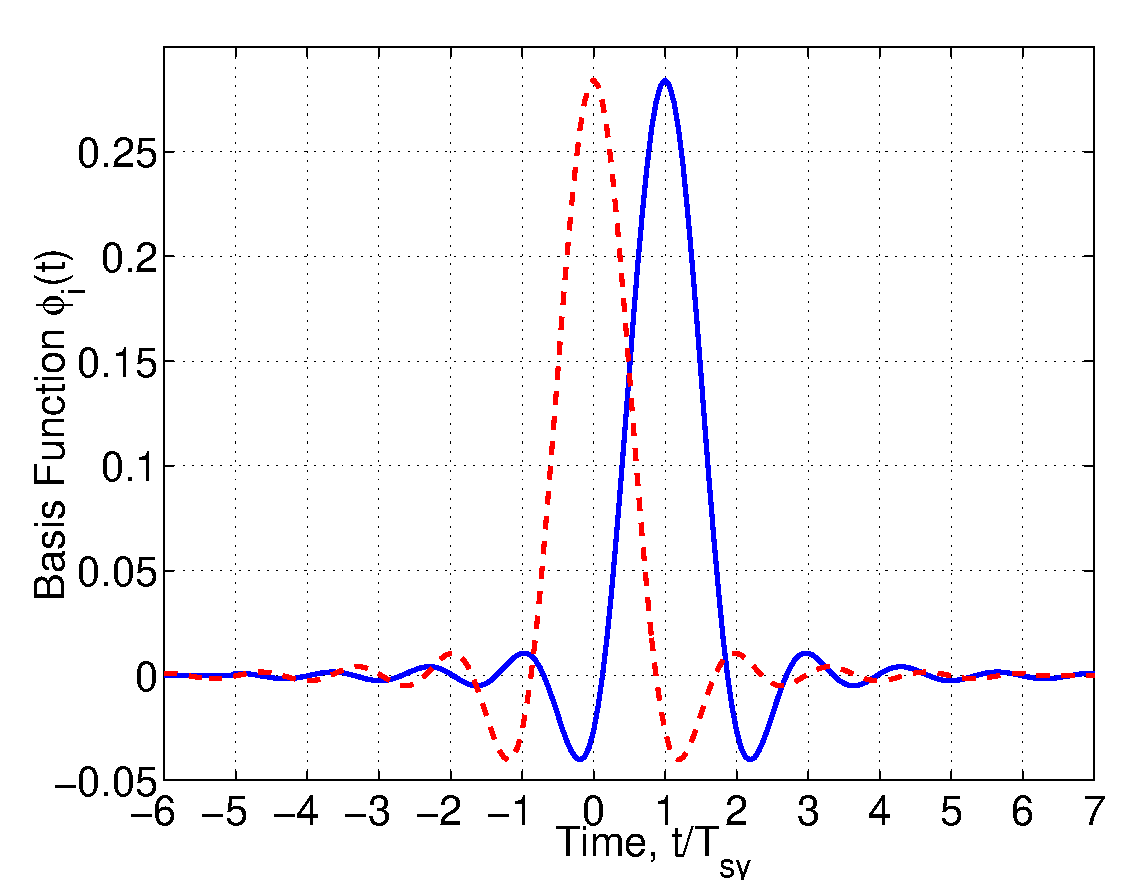
\includegraphics[width=0.6\textwidth]{../images/plotTwoTimeDelayedSRRCPulses.eps}}
  \caption{Two SRRC Pulses, delayed in time by $nT_{s}$ for any integer $n$, are orthogonal to each other.}
  \label{F:plotTwoTimeDelayedSRRCPulses}
\end{figure}

